%%%%%%%%%%%%%%%%%%%%%%%%%%%%%%%%%%%%%%%%%%%%%%%%%%%%%%%%%%%%%%%%%%%%%%
% LaTeX Template: Curriculum Vitae 
% Source: http://www.howtotex.com/
%%%%%%%%%%%%%%%%%%%%%%%%%%%%%%%%%%%%%%%%%%%%%%%%%%%%%%%%%%%%%%%%%%%%%%

\documentclass[paper=a4,fontsize=11pt]{scrartcl} % KOMA-article class
							
\usepackage[english]{babel}
\usepackage{graphicx}                    % Enable pdflatex
\usepackage[svgnames]{xcolor}            % Colors by their 'svgnames'
\usepackage{geometry}
	\textheight=650pt

\usepackage{hyperref}
\usepackage{color}
\usepackage{fontawesome}
\usepackage[export]{adjustbox}

\frenchspacing              % Better looking spacings after periods
\pagestyle{empty}           % No pagenumbers/headers/footers

%%% Custom sectioning (sectsty package)
%%% ------------------------------------------------------------
\usepackage{sectsty}

\sectionfont{%			            % Change font of \section command
	\usefont{OT1}{phv}{b}{n}%		% bch-b-n: CharterBT-Bold font
	\sectionrule{0pt}{0pt}{-5pt}{3pt}}

%%% Macros
%%% ------------------------------------------------------------
\newlength{\spacebox}
\settowidth{\spacebox}{8888888888}			% Box to align text
\newcommand{\sepspace}{\vspace*{1em}}		% Vertical space macro

\newcommand{\MyName}[1]{ % Name
		\Huge \usefont{OT1}{phv}{b}{n} \hfill #1
		\par \normalsize \normalfont}
		
\newcommand{\MySlogan}[1]{ % Slogan (optional)
		\large \usefont{OT1}{phv}{m}{n}\hfill \textit{#1}
		\par \normalsize \normalfont}

\newcommand{\NewPart}[1]{\section*{\uppercase{#1}}}

\newcommand{\PersonalEntry}[2]{
		\noindent\hangindent=0em\hangafter=0 % Indentation
		\parbox{\spacebox}{        % Box to align text
		\textit{#1}}		       % Entry name (birth, address, etc.)
		\hspace{2.5em} #2 \par}    % Entry value

\newcommand{\SkillsEntry}[2]{      % Same as \PersonalEntry
		\noindent\hangindent=0em\hangafter=0 % Indentation
		\parbox{\spacebox}{        % Box to align text
		\textit{#1}}			   % Entry name (birth, address, etc.)
		\hspace{2.5em} #2 \par}    % Entry value	

\newcommand{\EducationEntry}[4]{
		\noindent \textbf{#1} \hfill      % Study
		\colorbox{Black}{%
			\parbox{6em}{%
			\hfill\color{White}#2}} \par  % Duration
		\noindent \textit{#3} \par        % School
		\noindent\hangindent=2em\hangafter=0 \small #4 % Description
		\normalsize \par}

\newcommand{\WorkEntry}[4]{				  % Same as \EducationEntry
		\noindent \textbf{#1} \hfill      % Jobname
		\colorbox{Black}{\color{White}#2} \par  % Duration
		\noindent \textit{#3} \par              % Company
		\noindent\hangindent=2em\hangafter=0 \small #4 % Description
		\normalsize \par}

%%% ------------------------------------------------------------
\begin{document}

\begin{figure}
    \vspace*{60pt}
    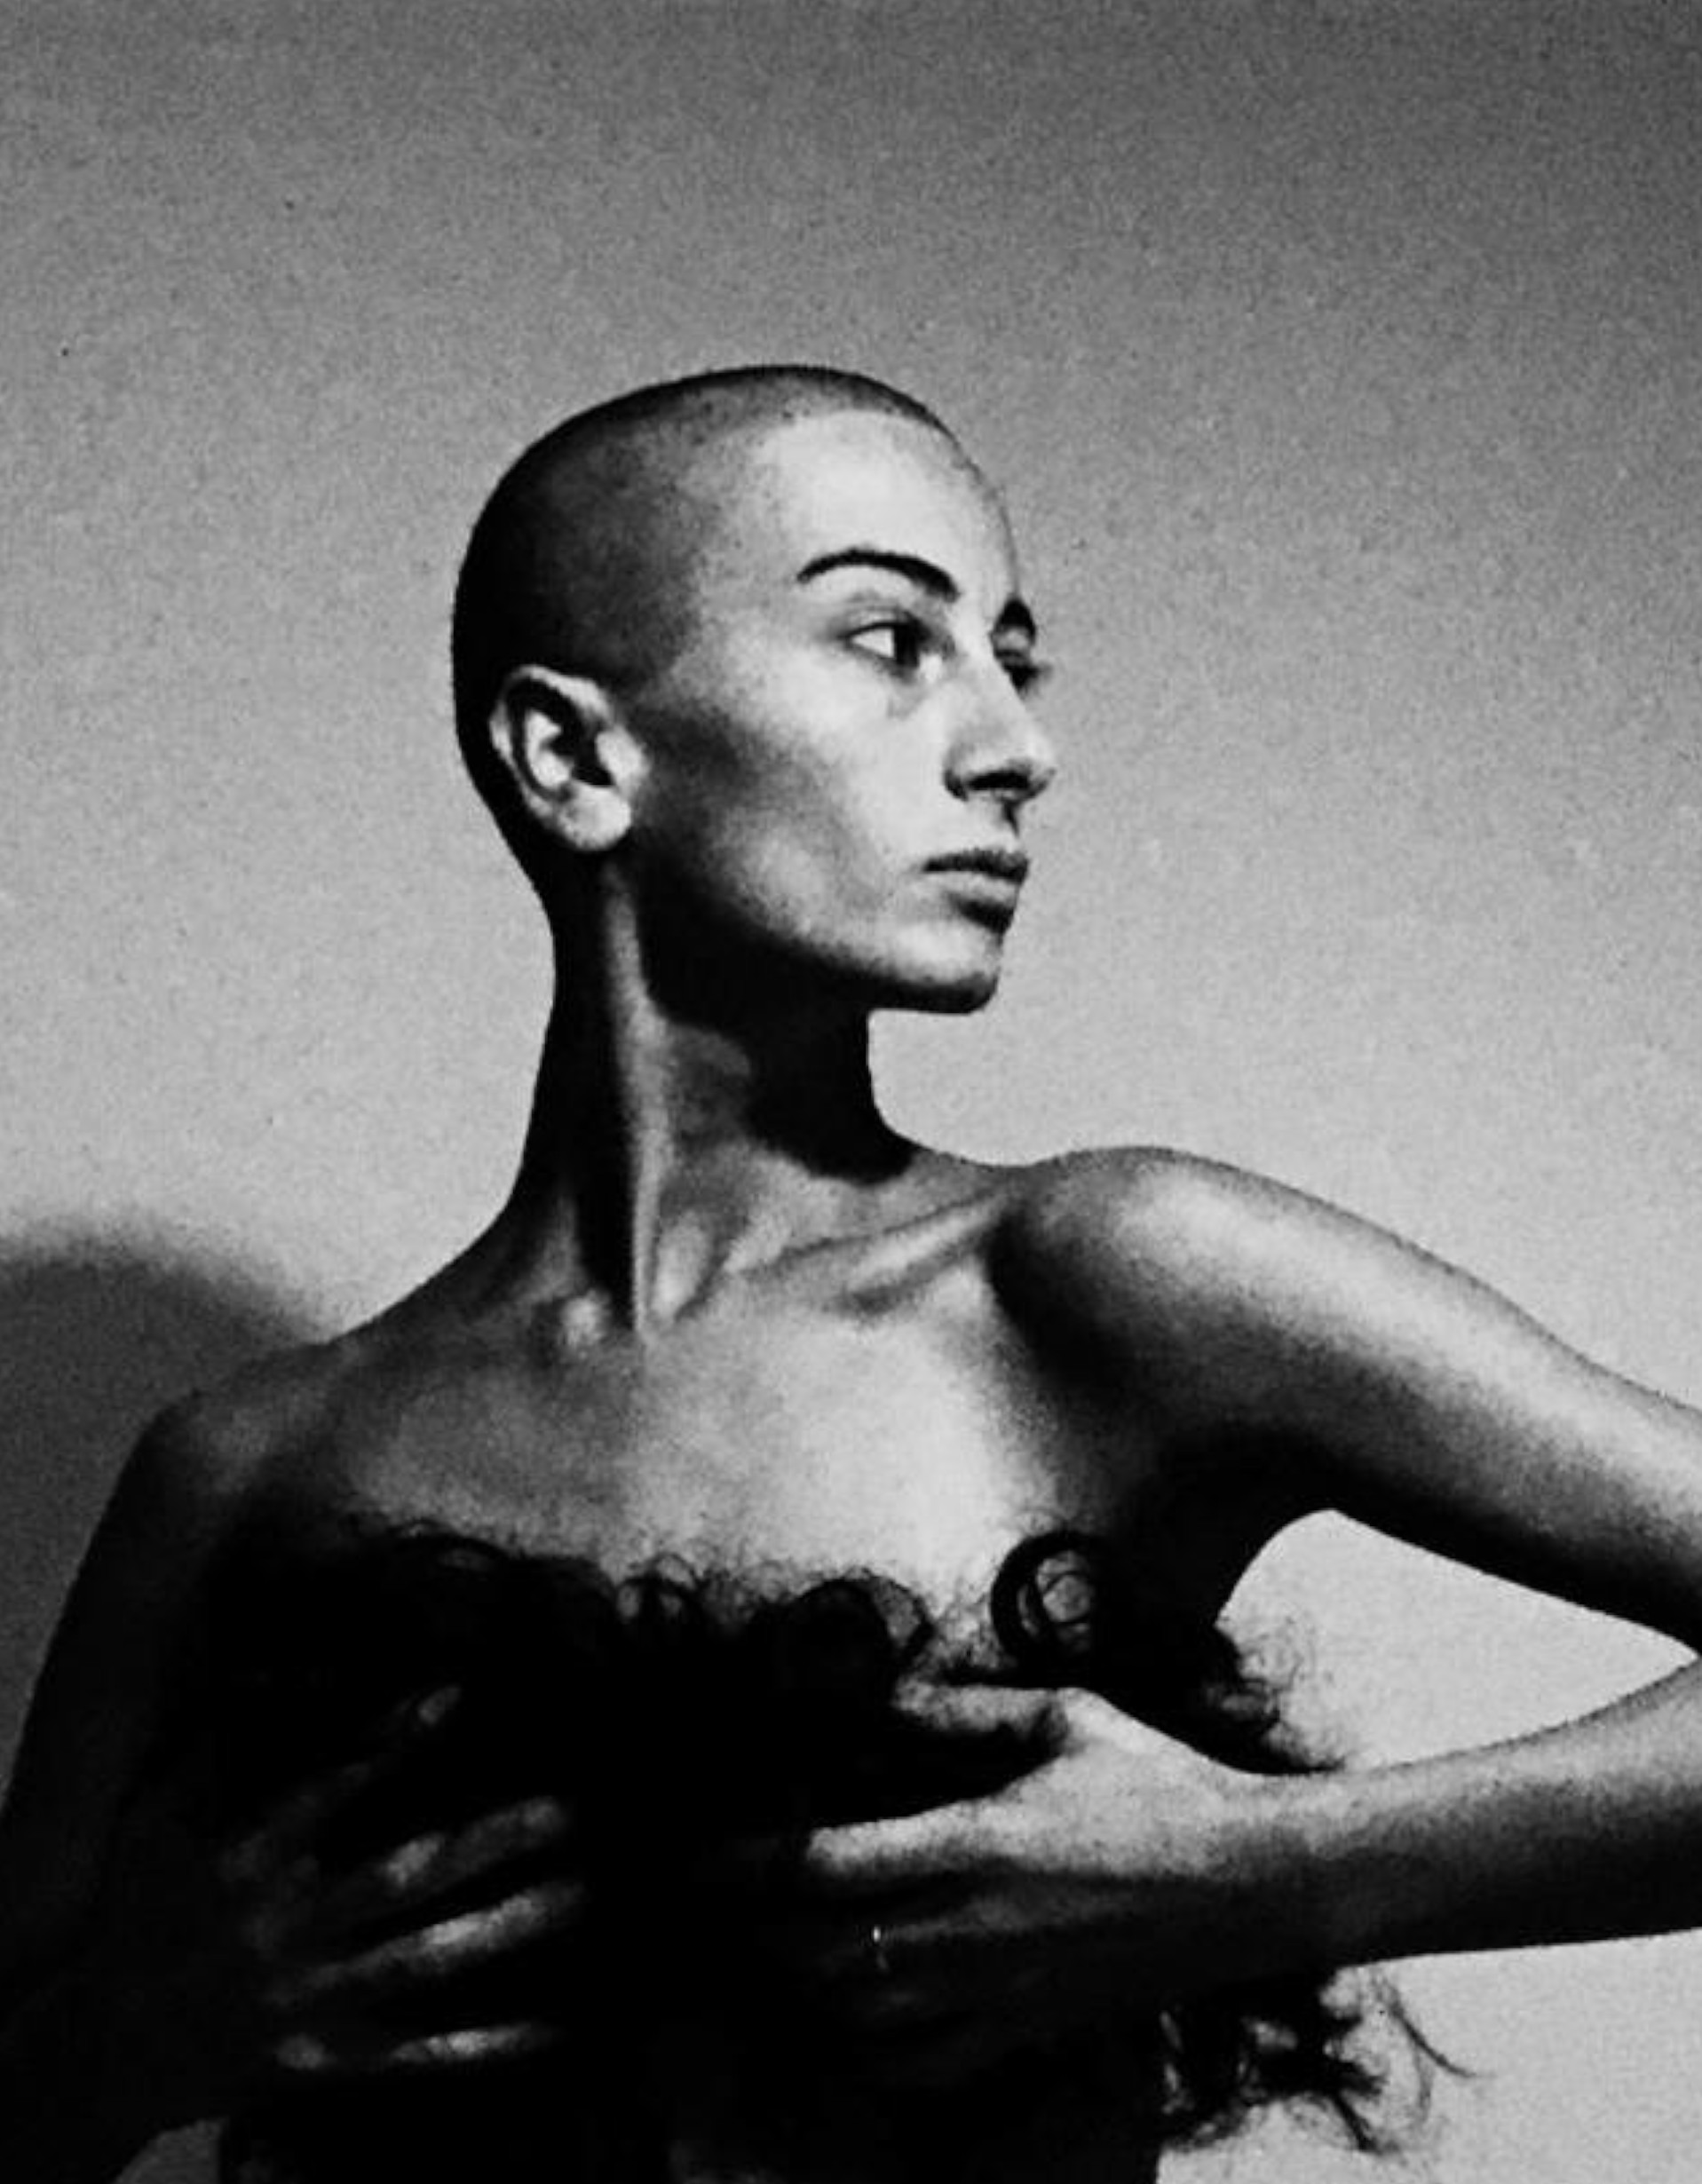
\includegraphics[width=100pt, left]{images/portrait}
    \vspace*{-30pt}
\end{figure}

\MyName{Simon Zimmermann}
\MySlogan{ArtistName: Hidonash} 

\sepspace

%%% ------------------------------------------------------------
\NewPart{Personal details}{}

\PersonalEntry{Birth}{June 5, 1993}
\PersonalEntry{Location}{Düsseldorf, Germany}
\PersonalEntry{Mail}{\href{mail@hidonash.com}{\color{red}mail@hidonash.com}}
\PersonalEntry{Website}{\href{https://www.hidonash.com}{\color{red}www.hidonash.com}}

%%% ------------------------------------------------------------
\NewPart{Education}{}

\EducationEntry{MSc. Media Informatics}{2018-2020}{University Of Applied Sciences Düsseldorf}{}
\sepspace
\EducationEntry{MSc. Music Informatics}{2018}{University Of Music Karlsruhe}{Guest Semester}
\sepspace
\EducationEntry{BEng. Media Engineering}{2012-2017}{University Of Applied Sciences Düsseldorf}{}
\newpage

%%% ------------------------------------------------------------
\NewPart{Projects}{}

\EducationEntry{Composer, Performer}{2016-2020}{"Exolar" - electronic music project with guitarist "Yannik Brehm}{Various self-managed independent digital releases}
\sepspace
\EducationEntry{Producer, Media-Artist}{2020}{"Computer Vision" - VR Experience for the song "Exolar - ComputerVision"} 
\sepspace
\EducationEntry{Composer, Producer}{2020}{"Hidonash - Yakiman" - released on "Soil Records"} 
\sepspace
\EducationEntry{Founder, Manager}{2021}{"system ctl" - independent event-series and label for electronic music} 
\sepspace
\EducationEntry{Composer, Producer}{2021}{"Hidonash - Verbose Liturgy" released on "Soil Records"} 
\sepspace
\EducationEntry{Founder, Manager}{2021-2022}{Various independent digital releases on "system ctl"} 
\sepspace

%%% ------------------------------------------------------------
\NewPart{Awards}{}

\EducationEntry{Composer, Producer}{2020}{Best contribution "!content" in the category Acoustic Stories, "Sound Cinema Düsseldorf"}
\sepspace

\EducationEntry{Composer, Producer}{2020}{Audience award for contribution "!content", "Sound Cinema Düsseldorf"} 

%%% ------------------------------------------------------------
\end{document}

